\section{Posición vehicular relativa}
La posición vehicular relativa se refiere a en qué lado de un vehículo A se encuentra un vehículo B. Es decir, si se toma como referencia el primer vehículo, en qué lado se encuentra el segundo; derecha, izquierda, delante o detrás.

El ''heading'' o rumbo, es la dirección hacia la que se está dirigiendo un vehículo con respecto al Norte (0 grados). En la figura \ref{figure:Bearing}, en el eje de coordenadas cartesiano. Cada vez que se realice una operación que involucre los ángulos, se emplea una función para mantenerlos en un rango de entre 0 a 360 grados.

El algoritmo \ref{alg:relative_vehicular_pos} mostrado se puede condensar en:
\begin{enumerate}
	\item Calcular el ángulo existente entre los dos vehículos, sin tener en cuenta la dirección del primer vehículo.
	\item Se resta el heading del vehículo de referencia al ángulo que hay entre los dos vehículos.
	\item Se contrasta con una serie de casos ya conocidos, y se devuelve el ángulo relativo [Imagen \ref{figure:VRP}].
\end{enumerate}

\begin{listing}
	\begin{minipage}{.4\textwidth}
		\begin{minted}[linenos=true]{javascript}
function calcularPosicionRelativa(heading, oLatitude, oLongitude, pLatitude, pLongitude) {
  var degrees = calculateAngleBetweenTwoPoints(oLatitude, oLongitude, pLatitude, pLongitude);
  var relativeAngle = correctDegrees(degrees - heading);

  var tmp = "";
  if (relativeAngle <= 15 || relativeAngle >= 345) {
    return "FRONT";
  } else if (relativeAngle >= 120 && relativeAngle <= 230) {
    return "BACK";
  } else if (relativeAngle < 120 && relativeAngle > 15) {
    return "LEFT";
  } else {
    return "RIGHT";
  }
}

function calcularAnguloEntreDosPuntos(ox, oy, x, y) {
  return toDegrees(Math.atan2(y - oy, x - ox));
}
		\end{minted}
	\end{minipage}
	\caption{Cálculo de la posición relativa vehicular.}\label{alg:relative_vehicular_pos}
\end{listing}

\begin{figure}[H]
	\begin{minipage}{.5\textwidth}
		\begin{center}
			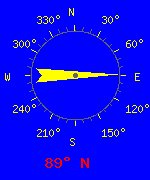
\includegraphics[scale=0.7]{bearing-1427303542791}
			\caption{Rumbo: el ángulo 0º está desplazado 90º con respecto al eje cartesiano.}
			\label{figure:Bearing}
		\end{center}
	\end{minipage}
	\begin{minipage}{.5\textwidth}
		\begin{center}
			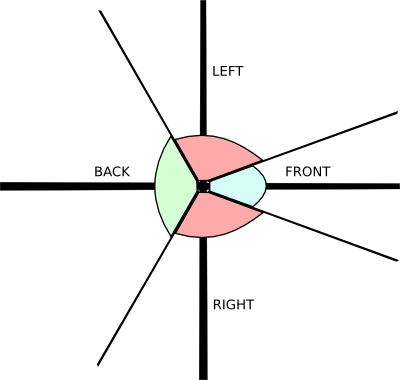
\includegraphics{relative_position2}
			\caption{Posición relativa vehicular.}
			\label{figure:VRP}
		\end{center}
	\end{minipage}
\end{figure}